% Line chart: Security level (x) vs Decaps instret (y) per variant
% Shows scaling behavior — log-log scale reveals power-law exponents
\tikzsetnextfilename{ch8-results-scaling-security-line}
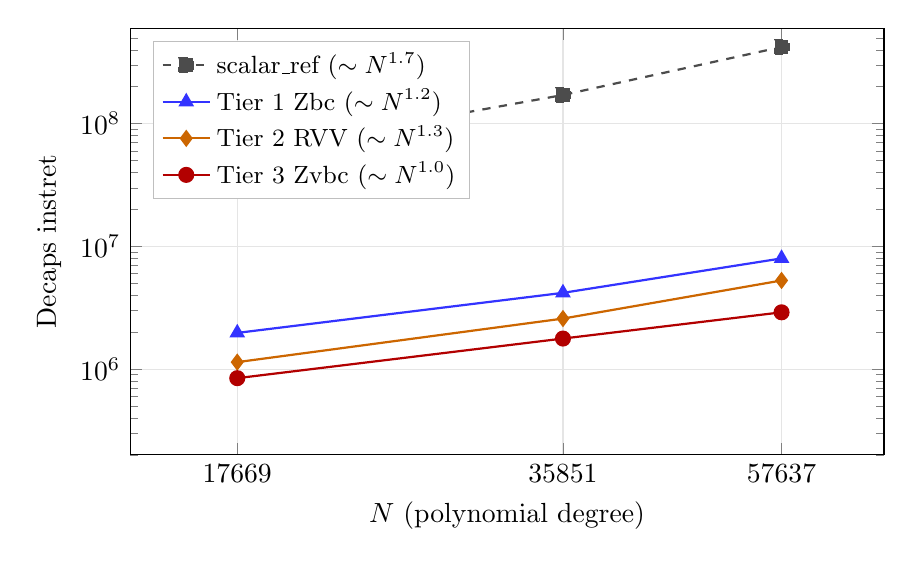
\begin{tikzpicture}
\begin{axis}[
  width=0.92\linewidth,
  height=7cm,
  xlabel={$N$ (polynomial degree)},
  ylabel={Decaps instret},
  xmode=log,
  ymode=log,
  log basis x=2,
  xtick={17669, 35851, 57637},
  xticklabels={\num{17669}, \num{35851}, \num{57637}},
  xmin=14000, xmax=72000,
  ymin=2e5, ymax=6e8,
  legend style={
    at={(0.03,0.97)},
    anchor=north west,
    font=\small,
    cells={anchor=west},
    draw=gray!50,
  },
  grid=major,
  grid style={gray!20},
  every axis plot/.append style={thick, mark size=2.5pt},
]

% scalar_ref: schoolbook O(N^2)
\addplot[color=black!70, mark=square*, dashed]
  coordinates {(17669, 56937074) (35851, 171349089) (57637, 421860950)};
\addlegendentry{scalar\_ref ($\sim N^{1.7}$)}

% Tier 1: Karatsuba Zbc
\addplot[color=blue!80, mark=triangle*]
  coordinates {(17669, 1972347) (35851, 4181542) (57637, 7980756)};
\addlegendentry{Tier~1 Zbc ($\sim N^{1.2}$)}

% Tier 2: Karatsuba RVV
\addplot[color=orange!80!black, mark=diamond*]
  coordinates {(17669, 1139356) (35851, 2579762) (57637, 5274100)};
\addlegendentry{Tier~2 RVV ($\sim N^{1.3}$)}

% Tier 3: Karatsuba Zvbc
\addplot[color=red!70!black, mark=*]
  coordinates {(17669, 843459) (35851, 1773770) (57637, 2902352)};
\addlegendentry{Tier~3 Zvbc ($\sim N^{1.0}$)}

\end{axis}
\end{tikzpicture}
